In this section, we report our simulation results and evaluate the efficiency of TDI (our program allocation algorithm) and point-based and index-based skyline computation algorithms discussed in previous sections of this paper. Our simulations are implemented in C\# with .NET Framework 4 (compatible with version2) and conducted on a machine of 3.4 GHz Intel Pentium 4 processor, 3 GB RAM, and Windows 7.

The simulations are ran with synthetic data-sets categorized as follows:

\begin{itemize}
\item Uniformed: data uniformly distributed in the data space of each
    attribute.
\item Rising: the attributes of the records are correlated to the first
    attribute of the data-set.
\item Falling: the attributes of the records are inversely correlated to
    the first attribute of the data-set.
\end{itemize}

In addition, we also conducted simulations of data-sets with varying \emph{record count} and \emph{dimensions}.  Record count ranges from 20,000 to 100,000, and dimensions ranges from 2 to 10. Our simulation are memory-only: at the started of a simulation, a data-set is loaded into memory from disk. Table~\ref{tab:sim_size} lists the size of data elements used in the implementation of the tuning time and index percentage simulation.

\begin{table}[h]
\caption{Simulation parameters.}
\label{tab:sim_size}
\centering
\begin{tabular}{l|c}
\hline
{\bf Item} & {\bf Size in Bytes}\\
\hline
Pointer of index ($ptr$) & 4\\
Field of record ($f$) & 8\\
Record/point ($p$) & $f \times n$\\
Minimal bounding rectangle (MBR) & $2 \times p$\\
Index entry ($E$) & MBR + $ptr$\\
\hline
\end{tabular}
\end{table}

\subsection{Dominance Tests}\label{sec:exp_dom_test}

\emph{Dominance tests} measures the number of record comparisons the client has to perform to evaluate a skyline query via Block-Nested-Loop (BNL)~\cite{conf/icde/BorzsonyiKS01}. A comparison determines if a record dominates another record. Comparisons are performed when a data bucket is downloaded. Intuitively, as the number of records in the a data-set increases, the number of dominance tests also increases.

Figure~\ref{fig:dt_rc} compares the the number of dominance tests of RPS and IPS with increasing data-set size, from $2\times10^4$ to $10\times10^4$ data records (with $n$ = 2 and $b$ = 10). \ref{fig:dt_rc_a} shows that both algorithms performs well. For the simulation with $6\times10^4$ records, only 4000 comparisons are performed. \ref{fig:dt_rc_a} shows that when skyline preference is ``opposite" of the ordering of data, the pruning is not as effective. For record count of $6\times10^4$, $2\times10^5$ comparisons are performed.

%Figure~\ref{fig:dt_rc} covers all cases of combinations of min and max attributes in 2-dimensional data for Point-Based (P-B) and Index-Based (I-P) skyline algorithms. Figure~\ref{fig:dt_rc_a} shows that the I-P algorithm performs better than I-B, and that I-P (min, min) performs the best. The performance is R-tree implementation dependent, and due to our implementation order, index entries based on the distance to the origin (min, min) skyline queries naturally perform better than other queries. Similarly, in Figure~\ref{fig:dt_rc_b}, the algorithm can prune very little due to the ordering of the MBRs; therefore, P-B and I-P based algorithms perform almost the same for (max, max) skyline queries.

Figure~\ref{fig:dt_dim} compares the number of dominance tests with increasing data dimensions. The experiments are conducted with the record count = 10,000, and a $b$ = 10. Figure~\ref{fig:dt_dim_a} compares the results when skyline query attribute specifiers are all min and all max. Figure~\ref{fig:dt_dim_b} shows the result of the number of dominance tests with different data types. The two figures show that as the number of data dimensions increases, the volume (or space) of the data also increases. This leads to more space for the records to ``hide" and not fall into the pruning region, and therefore the number of dominance tests increases.

%%
% Dominance Tests vs. Record Count
%%
\begin{figure}[!h]
  \centering
  \subfigure[\small (min, min) and (max, min)]{
    \label{fig:dt_rc_a}
    %\begin{minipage}[h!]{0.5\textwidth}
      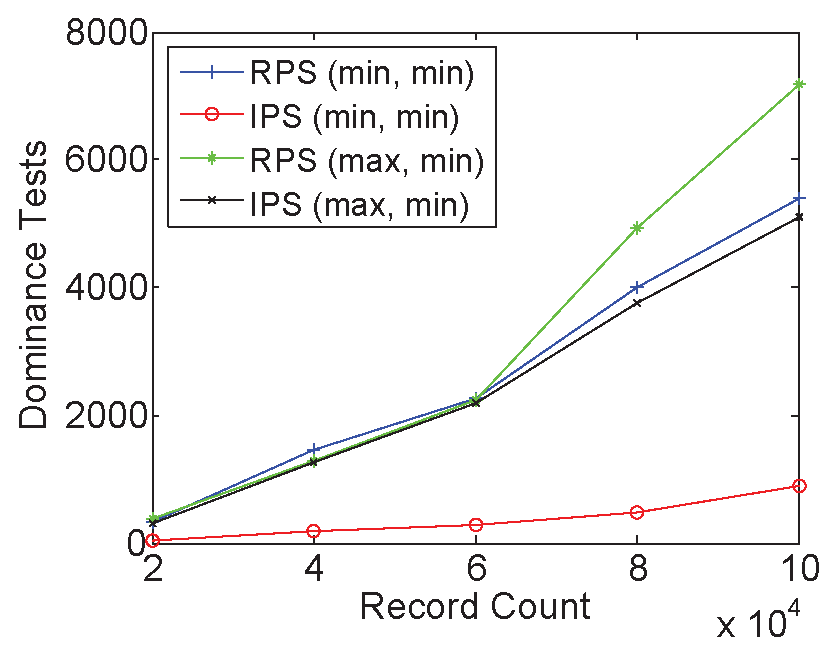
\includegraphics[width=2.5in]{Figures/exp/dt_rc_minmin_maxmin.eps}
    %\end{minipage}
    }
  \subfigure[\small (min, max) and (max, max)]{
    \label{fig:dt_rc_b}
    %\begin{minipage}[h!]{0.5\textwidth}
      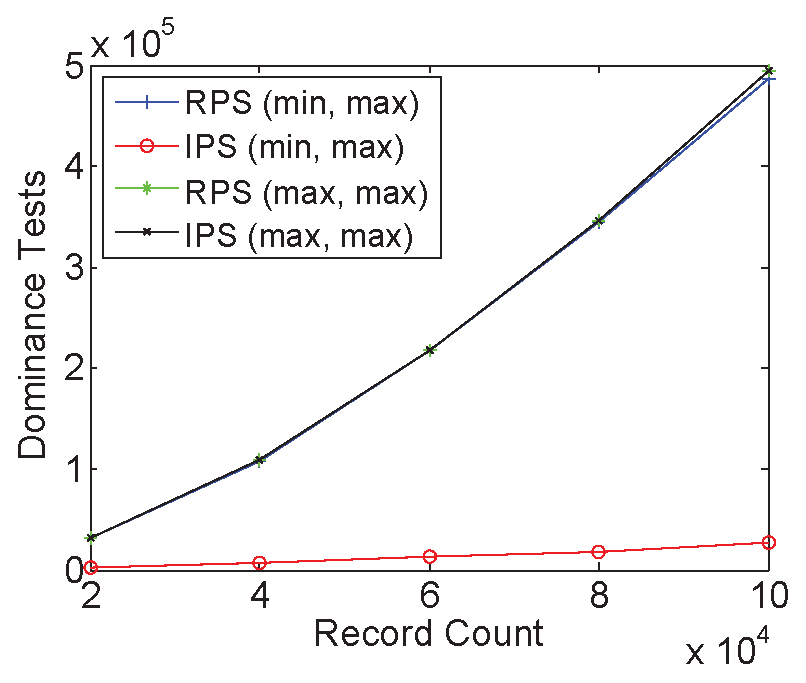
\includegraphics[width=2.5in]{Figures/exp/dt_rc_minmax_maxmax.eps}
    %\end{minipage}
    }
  \caption{\small Dominance Tests vs. Record Count. d = 2, b = 10,
  Data = uniformed}
  \label{fig:dt_rc}
\end{figure}


%%
% Dominance Test vs. Dimensions
%%
\begin{figure}[!h]
  \centering
  \subfigure[\small All Min and All Max. Data = uniformed]{
    \label{fig:dt_dim_a}
    %\begin{minipage}[h!]{0.5\textwidth}
      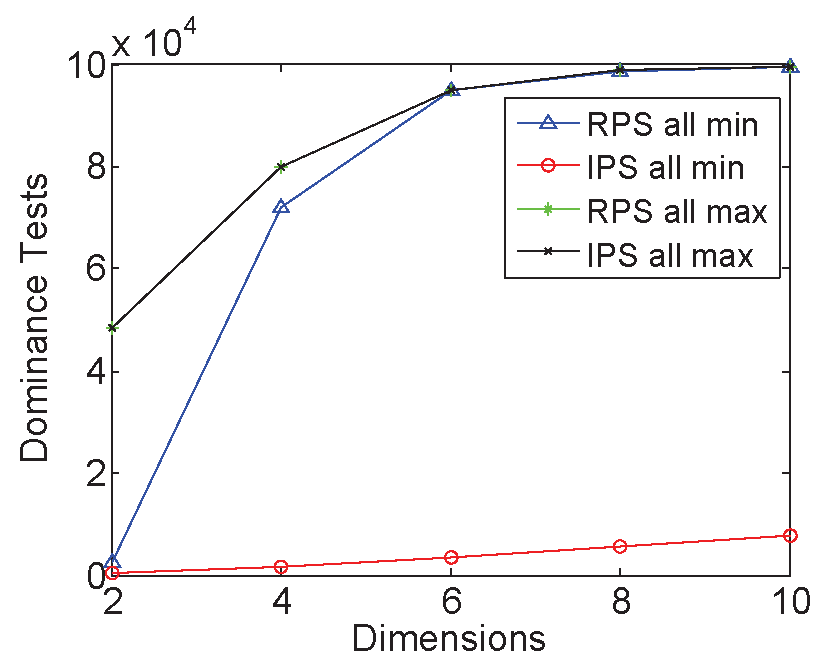
\includegraphics[width=2.5in]{Figures/exp/dt_dim_allmin_allmax.eps}
    %\end{minipage}
    }
  \subfigure[\small Mixed Data Types]{
    \label{fig:dt_dim_b}
    %\begin{minipage}[h!]{0.5\textwidth}
      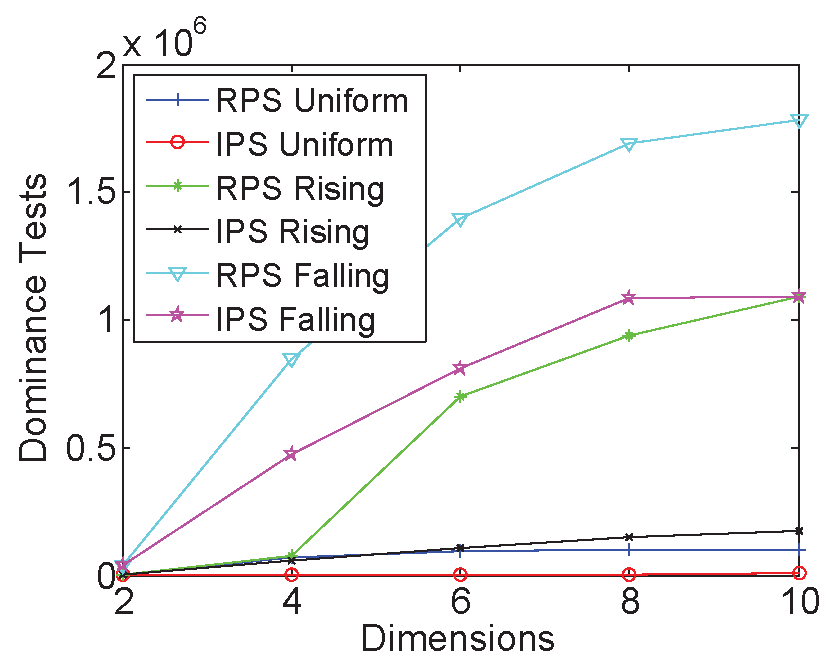
\includegraphics[width=2.5in]{Figures/exp/dt_dim_mixdata_rc10000.eps}
    %\end{minipage}
    }
  \caption{\small Dominance Tests vs. Dimensions. rc = 10000, b = 10}
  \label{fig:dt_dim}
\end{figure}


\subsection{Tuning Time}\label{sec:exp_tuning_time}

As discussed in Section~\ref{sec:wireless_broadcast}, tuning time is the total amount of data the client has to download to fulfill a skyline query. It is measured in bytes. The experiment simulates the creation of the TDI broadcast program by the server. Tuning time is found by simulating a client evaluation of a skyline query from the beginning of the cycle.

Figure~\ref{fig:tt_rec} illustrates tuning time versus increasing record count for all combinations of min and max attribute for 2-dimensional data. In all cases, the IPS performs several factors better than RPS.

Figure~\ref{fig:tt_dim} illustrates the simulation result for tuning time with increasing data dimension. The experiments are run with a record count = 10,000, and a $b$ = 10. Although the number of records stays the same, each additional dimension or data attribute of the data set adds space complexity to the data set. With increasing dimensionality, the cycle length also increases, as well as tuning time.

%%
% Tuning Time vs. Record Count
%%
\begin{figure}[!h]
  \centering
  \subfigure[\small (min, min) and (max, max)]{
    \label{fig:tt_rec_a}
    %\begin{minipage}[h!]{0.5\textwidth}
      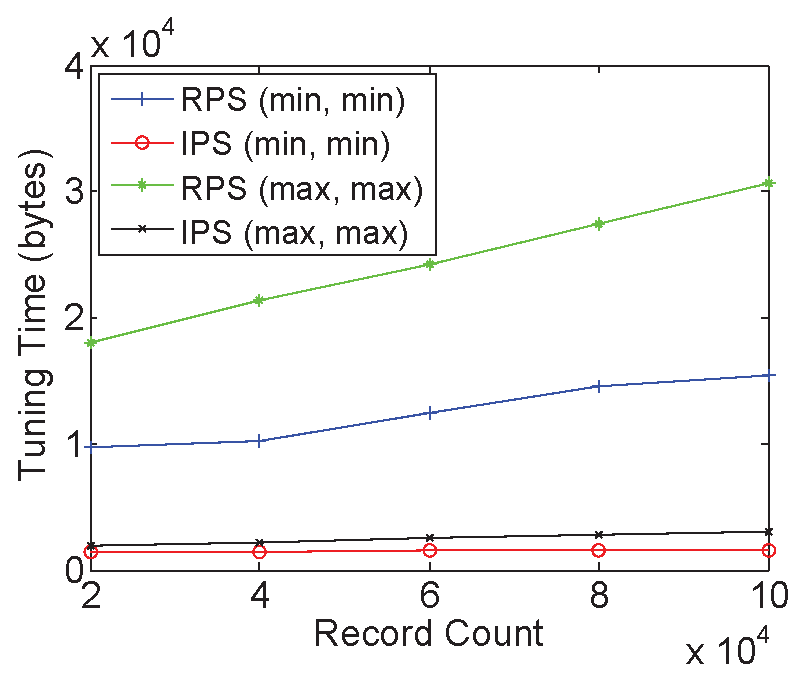
\includegraphics[width=2.5in]{Figures/exp/tt_rc_minmin_maxmax.eps}
    %\end{minipage}
    }
  \subfigure[\small (min, max) and (max, min)]{
    \label{fig:tt_rec_b}
    %\begin{minipage}[h!]{0.5\textwidth}
      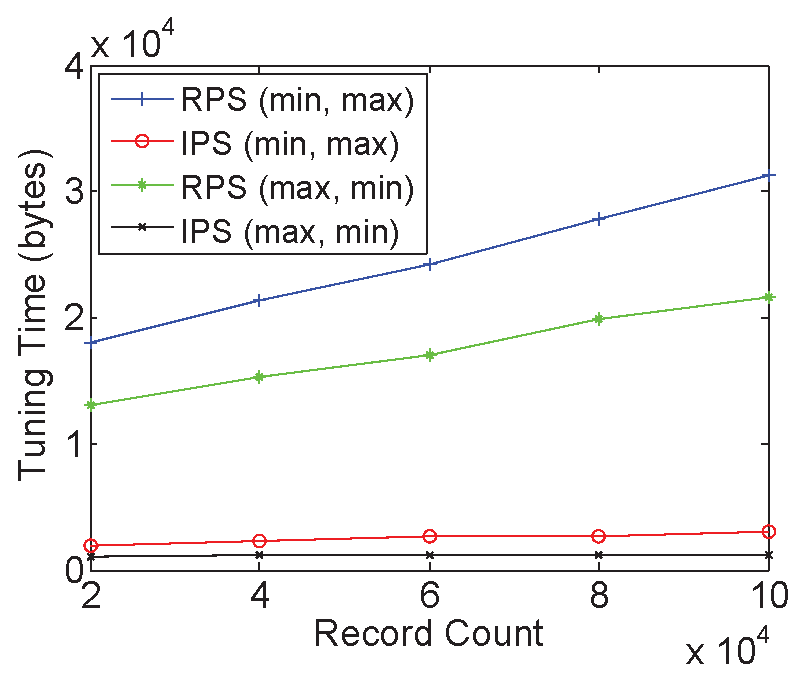
\includegraphics[width=2.5in]{Figures/exp/tt_rc_minmax_maxmin.eps}
    %\end{minipage}
    }
  \caption{\small Tuning Time vs. Record Count. d = 2, b = 10}
  \label{fig:tt_rec}
\end{figure}

%%
% Tuning Time vs. Dimension
%%
\begin{figure}[!h]
  \centering
  \subfigure[\small All Min and All Max]{
    \label{fig:tt_dim_a}
    %\begin{minipage}[h!]{0.5\textwidth}
      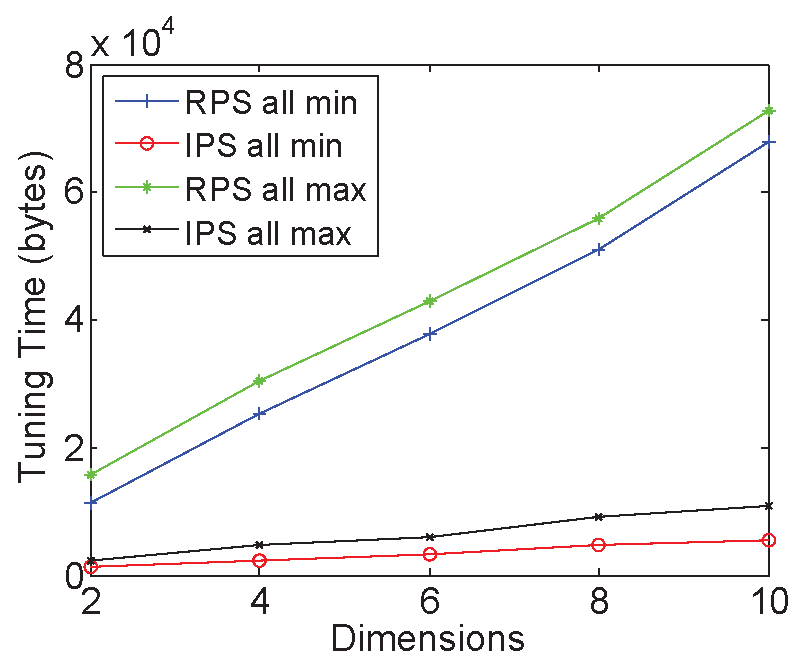
\includegraphics[width=2.5in]{Figures/exp/tt_dim_allmin_allmax_mod.eps}
    %\end{minipage}
    }
  \subfigure[\small Mixed Data Types]{
    \label{fig:tt_dim_b}
    %\begin{minipage}[h!]{0.5\textwidth}
      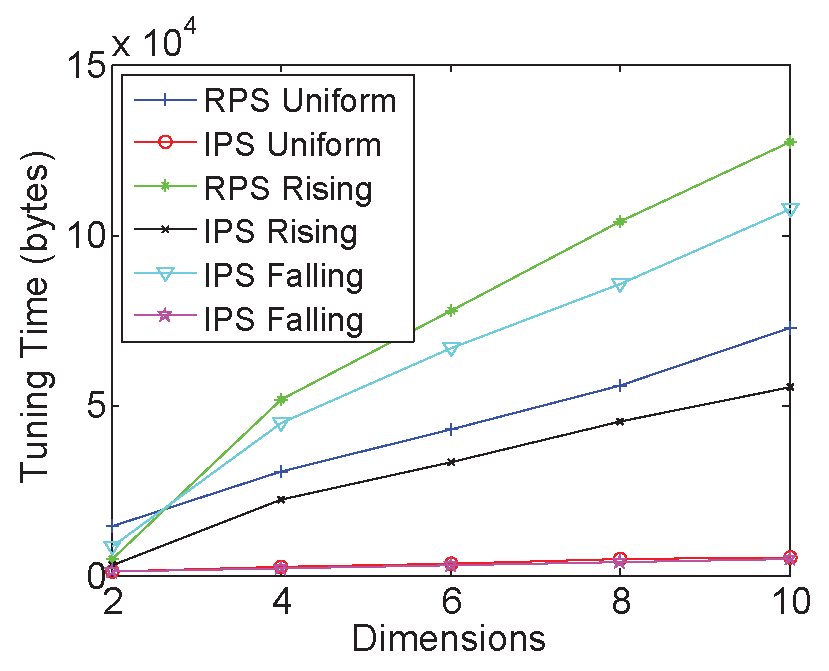
\includegraphics[width=2.5in]{Figures/exp/tt_dim_mixdata_rc10000.eps}
    %\end{minipage}
    }
  \caption{\small Tuning Time vs. Dimensionality. rc = 10000, b = 10}
  \label{fig:tt_dim}
\end{figure}

%%
% Index Percentage
%%
\begin{figure}[!h]
  \centering
  \subfigure[\small IP vs. Record Count]{
    \label{fig:ip_rc}
    %\begin{minipage}[h!]{0.5\textwidth}
      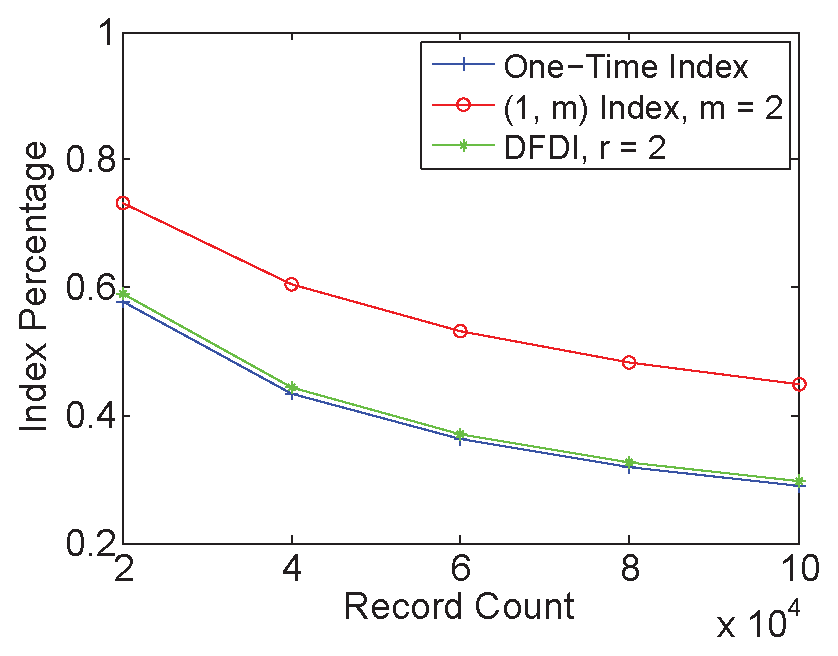
\includegraphics[width=2.5in]{Figures/exp/ip_rc.eps}
    %\end{minipage}
    }
  \subfigure[\small IP vs. Dimensionality]{
    \label{fig:ip_dim}
    %\begin{minipage}[h!]{0.5\textwidth}
      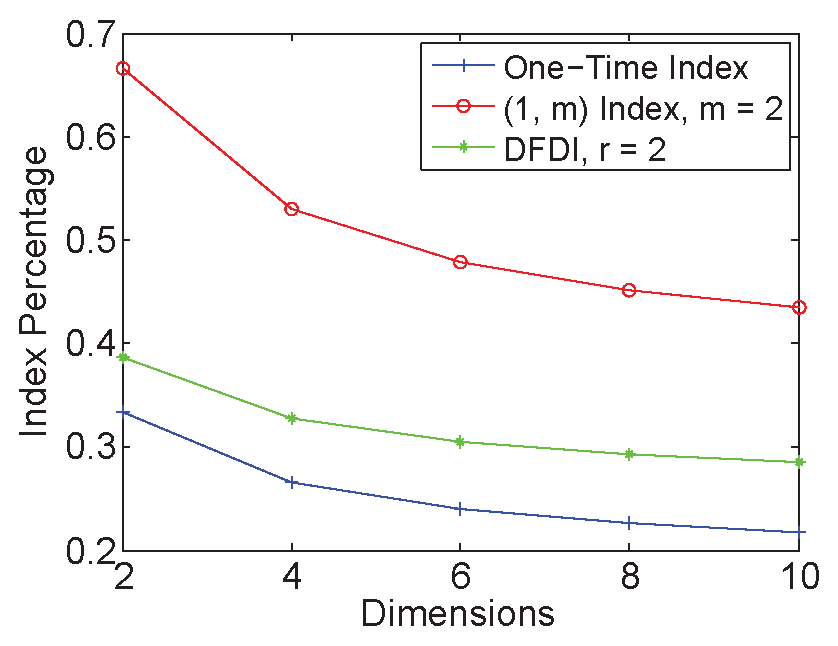
\includegraphics[width=2.5in]{Figures/exp/ip_dim.eps}
    %\end{minipage}
    }
  \caption{\small Index Percentage. b = 10}
  \label{fig:ip}
\end{figure}


\subsection{Index Percentage}

Index percentage measures the efficiency of the TDI broadcast program
allocation technique under increasing record count and increasing data
dimension. Index percentage is defined in
section~\ref{sec:wireless_broadcast}.

Figure~\ref{fig:ip_rc} shows index percentage versus increasing
record count. For the TDI, the simulation is run with a
replication level of 2, which means the root and the first level
below the root are replicated. For the (1, m) index, m = 2,
meaning the complete index is duplicated 2 times in the broadcast
cycle. The figure shows that the overhead of the index is high
when the number of records is low, but the overhead flattens as
the number of records grows. The one-time index is the baseline,
and as expected has the lowest index percentage. Although TDI
replicated the index for 2 levels, its index percentage is only
slightly (16\%) higher than the one-time index. This shows that
TDI is efficient in terms of space overhead, whereas the (1, m)
index has a far worse overhead for only 2 duplications.

Figure~\ref{fig:ip_dim} shows index percentage over increasing
data dimension. The experiment is conducted with 10,000 records
and a branching factor of 10. As the data size grows with the
number of dimensions, the index is only slightly affected by the
growth. The size of the index grows because it needs extra space
to store the information of the extra dimensions, but the tree
height is largely unaffected; thus gives the falling of index
percentage with growing dimension.

%Simulate 3 algorithms:
%\begin{enumerate}
%\item R-Tree one-time index \item R-Tree TDI \item Grid R-Tree
%TDI
%\end{enumerate}

%Measurements:
%\begin{enumerate}
%\item Index percentage (with variable branching factor) \item
%Tuning time (with variable branching factor) \item Dominance tests
%(with variable branching factor)
%\end{enumerate}
